\documentclass[11pt]{article}
\usepackage[letterpaper,margin=0.8in]{geometry}
\usepackage{epic}
\usepackage{eepic}
\usepackage{graphicx}
\usepackage{algorithm,algorithmic}
 \usepackage{enumitem}
\usepackage{amsfonts,mathrsfs}
\usepackage{hyperref}
\usepackage{color}
\usepackage{geometry}
\usepackage{changepage}
\usepackage{amsmath}
\pagestyle{empty}
\setlength{\textheight}{9.5in}
\usepackage {tikz}
\usetikzlibrary{shapes,arrows, positioning}
\usepackage{caption}
\DeclareMathOperator{\E}{\mathbb E}
\DeclareMathOperator*{\argmax}{argmax}


\begin{document}
\setlength{\fboxrule}{.5mm}\setlength{\fboxsep}{1.2mm}
\newlength{\boxlength}\setlength{\boxlength}{\textwidth}
\addtolength{\boxlength}{-4mm}
\begin{center}\framebox{\parbox{\boxlength}{\bf
Robot Learning \hfill Assignment 2\\
CS 4756 Spring 2025 \hfill Due 11:59pm Friday, February 28}}\end{center}
\vspace{5mm}
\setlength{\fboxrule}{0.1pt}\setlength{\fboxsep}{2mm}

\def\ind{\hspace*{0.3in}}
\def\gap{0.2in}
\noindent{\bf (1) Policy Gradients (10 points)} 
\vskip \gap
\noindent\fbox{%
\parbox{\textwidth}{%
\noindent \emph{Recap:} Recall that the goal of RL is to learn some $\theta^*$ that maximizes the objective function:
\begin{equation}\label{eq:1}
    J(\theta) = 
\mathbb{E}_{\tau \sim \pi_{\theta}(\tau)}\big[r(\tau)\big]
\end{equation}
where each $\tau$ is a rollout of length $T_\tau$ and $r(\tau) = \sum_{t = 0}^{T_\tau-1} r(s_t, a_t)$ is the reward for that rollout. $\pi_\theta(\tau)$ is the probability of the rollout under policy $\pi_\theta$, i.e. $\pi_\theta(\tau) = \Pr[s_0] \pi_\theta(a_0 | s_0)\prod_{t = 1}^{T_\tau-1} \Pr[s_t | s_{t-1}, a_{t-1}]\pi_\theta(a_t | s_t)$.
\newline

\noindent The policy gradient approach requires that we take the gradient of this objective as follows:
\begin{align}\label{eq:6}
    \nabla_{\theta}J(\theta) &= \nabla_{\theta}\int \pi_{\theta}(\tau)r(\tau) \ d\tau
    = \int \pi_{\theta}(\tau)
    \nabla_{\theta}
    \log \pi_{\theta}(\tau)r(\tau) \ d\tau\\
    &= \mathbb{E}_{\tau \sim \pi_\theta(\tau)} \big[ \nabla_{\theta}
    \log \pi_{\theta}(\tau)r(\tau)
    \big] \label{eq:4}
\end{align}

The gradient can further be refined by noting that future actions do not affect past rewards (the causality assumption), resulting in the following ``reward-to-go" formulation:

\begin{equation}\label{eq:5}
    \nabla_\theta J(\theta) &=  \E_{\tau\sim\pi_\theta(\tau)}\left[\sum_{t = 0}^{T_\tau-1}\left(\nabla_\theta \log \pi_\theta(a_t | s_t) \cdot \sum_{t' = t}^{T_\tau-1}r(s_{t'}, a_{t'})\right)\right]
\end{equation}
}%
}

\vskip \gap
\noindent In this question, we consider a toy MDP and get familiar with computing policy gradients.
\newline


\noindent{\bf (a)} 
Show the following step in \ref{eq:6} holds true and explain why this step is valid.:

$$\nabla_{\theta}\int \pi_{\theta}(\tau)r(\tau) \ d\tau
    = \int \pi_{\theta}(\tau)
    \nabla_{\theta}
    \log \pi_{\theta}(\tau)r(\tau) \ d\tau$$


\noindent{\bf (b)} 
Starting from Equation \ref{eq:4}, use the causality assumption (that future actions do not affect past rewards) to derive the "reward-to-go" formulation given in Equation \ref{eq:5}. Show the intermediate steps.
\newline

\noindent {\bf (c)} 
We introduce a baseline to reduce the variance of the policy gradient estimator \( b(s_t) \), leading to the advantage function:
\[
A^{\pi_{\theta}}(s_t, a_t) = Q^{\pi_{\theta}}(s_t, a_t) - V^{\pi_{\theta}}(s_t)
\]

\noindent Prove that subtracting a baseline does not introduce bias in the gradient estimation, i.e., show that:
\begin{equation}
\nabla_\theta J(\theta) = \mathbb{E}_{\tau \sim \pi_\theta(\tau)} \left[\sum_{t=0}^{T_\tau - 1} \nabla_\theta \log \pi_\theta(a_t | s_t) \cdot A(s_t, a_t)\right]
\end{equation}
Explain why the expectation of the baseline term vanishes.

\noindent \textit{Hint}:  
\begin{itemize}
    \item \textbf{}  
    Show that adding \( b(s_t) \) does not affect the expected gradient by proving its expectation is zero.
    \item \textbf{}  
    Rewrite the policy gradient with the bias and show that it does not change the expectation
\end{itemize}




\noindent Now, consider the following infinite-horizon MDP. 

\begin{figure}[h!]
\centering
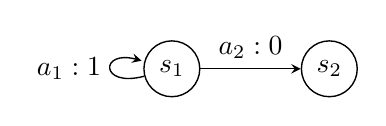
\begin{tikzpicture}[->,>=stealth, line width = 0.5 pt,node distance = 2 cm]

\node [circle, draw] (one) {$s_1$};
\node [circle, draw] (two) [right of=one] {$s_2$};
\path (one) edge [loop left] node  {$a_1:1$}(one);
\path (one) edge node [above, sloped] {$a_2:0$} (two);
--\end{tikzpicture}
\end{figure}

\noindent The initial state is always $s_1$, and the episode terminates when $s_2$ is reached. The agent receives reward 1 for taking action $a_1$ and reward 0 for taking action $a_2$. In this case, we can define the policy with a single parameter $\theta$:
$$\pi_{\theta}(a_1|s_1) = \theta, \ \ \ \pi_{\theta}(a_2|s_1) = 1-\theta$$
\newline

\noindent \( J(\theta) = \mathbb{E}_{\tau \sim \pi_{\theta}} [R(\tau)] \), and by the policy gradient method,

\[
\nabla_{\theta} J(\theta) = \mathbb{E}_{\tau \sim \pi_{\theta}} \left[ (\nabla_{\theta} \log \pi_{\theta}(\tau)) \cdot R(\tau) \right]
\]

\noindent Here, \( \tau \) is a trajectory \( s_0, a_0, ..., s_T, a_T \) that terminates after \( T + 1 \) steps.  

\noindent And, \( R(\tau) = \sum_{t=0}^{T} r(s_t, a_t) \), and 

\[
\pi_{\theta}(\tau) = p(s_0) \pi_{\theta}(a_0 | s_0) \prod_{t=1}^{T} p(s_t | s_{t-1}, a_{t-1}) \pi_{\theta}(a_t | s_t).
\]

\noindent{\bf (d)} 
Using the policy gradient theorem and the definition of our policy, compute the gradient of the expected return of $\pi_\theta$ with respect to the parameter $\theta$ (Eq. \ref{eq:4}). Do not use discounting. The sum should telescope to a closed form solution.
\newline
You may find this fact useful:
$$\sum^{\infty}_{k=1}k\alpha^{k-1} = \frac{d}{d\alpha}\sum^{\infty}_{k=1}\alpha^{k} $$
\newline
\noindent{\bf (e)} Compute the expected return of the policy $\pi_\theta$ directly using the law of total expectation(Eq. \ref{eq:1}). Compute the gradient of this expression and verify that it matches your result in {\bf (d)}.
\newline

\noindent{\bf (f)} Reward-to-go can be helpful and improve the statistical qualities of our policy gradient. Apply reward-to-go as an advantage estimator. Write the new policy gradient (Eq. \ref{eq:5}), and verify that it is unbiased.

\newpage

\vskip \gap \noindent{\bf (2) Reward Shaping with an Approximate Value Function (5 points)} 
\newline

\noindent Previously, we saw how acting greedily with an approximate value function can result in a \emph{worse} policy. Instead, what if we use the approximate value function to \emph{shape the reward}? 
\newline


\noindent Let's define a \emph{reward bonus} using the approximate value function from Q2. 

$$F(s,s') = \gamma \hat V(s') - \hat V(s)$$

\noindent This extra reward is gained whenever we transition from state $s$ to state $s'$. 
Informally, we are giving a small intermediate reward for moving toward states of higher value. Adding these intermediate rewards helps in speeding up a policy's convergence in environments with sparse rewards.

\noindent At each step $i$ of an episode, the shaped reward $R_i$ is then defined as
$$R_i = r_i + F(s_i,s_{i+1})$$
where $r_i$ is the base reward $r(s_i, a_i)$ received for step $i$. We continue to use a \emph{discount factor} of $\gamma$ in computing total reward. Recall that for an infinite-horizon setting, the total cumulative reward is typically expressed as:

$$R = \sum_{i = 0}^{\infty} \gamma^i r_i$$

\noindent In this problem, we will explore how this changes when shaping the reward with the approximate value function.
\newline


\noindent{\bf (a)} \noindent Consider a given episode of potentially infinite-length, of visited states $s_0, s_1,...$ 

\noindent Write out the total reward received in the shaped environment, expressed in terms of the total reward that would have been accrued in the unshaped environment. What is noticeable about this relationship? 
\newline

\noindent{\bf (b)} The policy $\hat \pi$ is found by optimizing the shaped rewards, while the policy $\pi^*$ is found by optimizing the unshaped rewards. Although the policies are derived using different reward structures, we ultimately want to compare their performance using the same value function.
\newline

\noindent Explain why the performance of the optimal policy $\hat \pi$ computed with the shaped rewards is the same as the performance of the optimal policy $\pi^*$ computed with the unshaped rewards. Specifically, explain why:

$$||V^{\pi^*} - V^{\hat \pi}||_{\infty} = 0$$

\noindent \textit{Hint:} Use your interpretation from part (a) to reason about why the performance is unaffected by reward shaping. You can either use the math or provide an explanation based on the takeaway from part (a).





\newpage
\vskip \gap \noindent{\bf (3) (Mandatory for 5756): Off Policy Gradient Estimation (10 points)}
\newline

In this problem, you will work towards deriving the off-policy gradient of a policy using importance weighting techniques. Consider a finite-horizon MDP $\mathcal{M} = \{ \mathcal{S}, \mathcal{A}, P, R, H, \mu_0 \}$, with a policy $\pi_{\theta}$ that we want to optimize, and a different policy $\pi'$ that generates the trajectory data. 

The trajectory $\tau = \{s_0, a_0, s_1, a_1, \dots, s_{H-1}, a_H \}$ is sampled using the policy $\pi'$, and the objective is to compute the gradient of $\pi_{\theta}$ using this off-policy data. The reward function is defined as the sum of rewards over the trajectory, \( R(\tau) = \sum_{t=0}^{H-1} r(s_t, a_t) \), and the goal is to maximize the expected cumulative reward. Recall that the gradient of the objective function can be expressed as:

\[
\nabla_{\theta} J(\theta) = \mathbb{E}_{\tau \sim \pi_{\theta}} \left[ \nabla_{\theta} \log \pi_{\theta}(\tau) R(\tau) \right]
\] where $ \pi_{\theta}(\tau) = \mu_0(s_0) \prod_{t=0}^{H-1} \pi_{\theta}(a_t|s_t) P(s_{t+1}|s_t, a_t) $.

Since the data is collected under a different policy $\pi'$, we need to use importance weighting to correct for the distribution mismatch. This will allow us to estimate the policy gradient for $\pi_{\theta}$ using data collected from $\pi'$.
\newline

\noindent{\bf (a)} Show that the policy gradient can be written using importance weights as:
\[
\nabla_{\theta} J(\theta) = \mathbb{E}_{\tau \sim \pi'} \left[ \frac{\pi_{\theta}(\tau)}{\pi'(\tau)} \nabla_{\theta} \log \pi_{\theta}(\tau) R(\tau) \right]
\]

\noindent \textit{Hint:} Multiply and divide by $\pi'(\tau)$, and use the fact that the expectation over $\pi_{\theta}$ can be transformed into an expectation over $\pi'$ using importance sampling.
\newline

\noindent{\bf (b)} Derive an expression for the ratio $\frac{\pi_{\theta}(\tau)}{\pi'(\tau)}$ in terms of the individual action probabilities $\pi_{\theta}(a_t|s_t)$ and $\pi'(a_t|s_t)$ for $t = 0, \dots, H-1$.
\newline

\noindent \textit{Hint:} Use the fact that the probability of a trajectory is the product of action probabilities and transition probabilities under the respective policies.
\newline

\noindent{\bf (c)} Now, derive an expression for $\nabla_{\theta} \log \pi_{\theta}(\tau)$ in terms of $\nabla_{\theta} \log \pi_{\theta}(a_t|s_t)$ for $t = 0, \dots, H-1$.
\newline

\noindent{\bf (d)}
What are the key benefits of using importance weighting to estimate the gradient of a target policy $\pi_\theta$ using data collected under a different policy $\pi'$? Why is it useful in practical settings?

\end{document}
